\pdfminorversion=4
\documentclass[xcolor=dvipsnames,hyperref={pdfpagelabels=false},unknownkeysallowed]{beamer}
\usepackage{tabls}
\usepackage{picture}
\usepackage{graphicx}
\usepackage{tcolorbox}
\usepackage{subcaption}
\captionsetup{compatibility=false}
%\usepackage{animate}

%To add a grid to the slides for aligning stuff
%\usepackage[texcoord,grid,gridunit=mm,gridcolor=gray,subgridcolor=gray!10,gridBG=true]{eso-pic}



%Tikz stuff
\usepackage{tikz}
\usetikzlibrary{shapes.geometric, arrows,shapes.arrows,calc,positioning}
\tikzstyle{startstop} = [rectangle, rounded corners, minimum width=2cm, text
    width=1.8cm, minimum height=1cm,text centered, text=white,draw=black, fill=Gray!140]
\tikzstyle{io} = [trapezium, trapezium left angle=70, trapezium right angle=110,
minimum width=0.5cm, minimum height=1cm, text centered, draw=black,
fill=blue!20!Gray!90!,text=white]
\tikzstyle{process} = [rectangle, minimum width=2cm, minimum height=1cm, text
centered, text width=2cm, draw=black, text=white,fill=Gray!140!blue!70!white]
\tikzstyle{decision} = [diamond, minimum width=2.0cm, minimum
    height=0.81cm,aspect=1.40, text centered, draw=black, fill=Gray!,text=white]
\tikzstyle{arrow} = [thick,line width=0.5mm,->,>=stealth]
\tikzstyle{arrow1} = [dashed,->,>=stealth]


\tikzset{>=stealth}

\newcommand{\tikzmark}[3][]{\tikz[overlay,remember picture,baseline] \node [anchor=base,#1](#2) {\ensuremath{#3}};}
\newcommand{\FOM}{\text{FOM}}






\usepackage[absolute,overlay]{textpos}

\newdimen\pc \pc=14bp
\def\XY#1#2{\xy{#1\pc}{#2\pc}}

\newcommand\myblock[3]{%
    \begin{textblock*}{\paperwidth}(#1\paperwidth,#2\paperwidth)
        \raggedright #3\hspace{0.5em}
    \end{textblock*}}



\definecolor{myblue}{rgb}{0.7, 0.7, 60.0}
\definecolor{mylightblue}{rgb}{1,1,1}
\newcommand*{\boxedcolor}{blue}
\makeatletter
\renewcommand{\boxed}[1]{\textcolor{\boxedcolor}{%
  \fbox{\normalcolor\m@th$\displaystyle#1$}}}
\makeatother

\newcommand{\highlight}[1]{%
    \colorbox{myblue!50}{\ensuremath{\displaystyle#1}}}

\renewcommand{\u}[1]{\underline{#1}}

\newcommand{\iso}[2]{${}^{{#2}}${#1} }
\newcommand{\nubar}[0]{\ensuremath{\overline{\nu}} }
\newcommand{\keff}[0]{\ensuremath{{k}_{\textsf{eff}}} }
\newcommand{\sa}[0]{\ensuremath{\sigma_c} }
\newcommand{\sfiss}[0]{\ensuremath{\sigma_f} }
\newcommand{\st}[0]{\ensuremath{\sigma_t} }
\newcommand{\ds}[0]{\displaystyle}
\newcommand{\expect}[1]{E[#1] }
\newcommand{\colg}[1]{{\color{ForestGreen} #1}}
\newcommand{\coly}[1]{{\color{yellow} #1}}
\newcommand{\colb}[1]{{\color{blue} #1}}
\newcommand{\colG}[1]{{\color{Gray!110} #1}}
\newcommand{\colr}[1]{{\color{red} #1}}
\usepackage{amsfonts}
\newlength{\wideitemsep}
\newlength{\tabsep}
\setlength{\tabsep}{0.99cm}
\setlength{\wideitemsep}{8pt}
\addtolength{\wideitemsep}{5pt}
\let\olditem\item
\renewcommand{\item}{\setlength{\itemsep}{\wideitemsep}\olditem}

\newcommand{\N}{\mathbb{N}}
\newcommand{\Z}{\mathbb{Z}}
\newcommand{\deriv}[2]{\frac{\mathrm{d} #1}{\mathrm{d} #2}}
\newcommand{\pderiv}[2]{\frac{\partial #1}{\partial #2}}
\newcommand{\bx}{\mathbf{X}}
\newcommand{\ba}{\mathbf{A}}
\newcommand{\by}{\mathbf{Y}}
\newcommand{\bj}{\mathbf{J}}
\newcommand{\bs}{\mathbf{s}}
\newcommand{\B}[1]{\ensuremath{\mathbf{#1}}}
\newcommand{\Dt}{\Delta t}
\renewcommand{\d}{\mathsf{d}}
\newcommand{\mom}[1]{\langle #1 \rangle}
\newcommand{\cur}[1]{\left\{ #1 \right\}}
\newcommand{\xl}{{x_{i-1/2}}}
\newcommand{\xr}{{x_{i+1/2}}}
\newcommand{\il}{{i-1/2}}
\newcommand{\ir}{{i+1/2}}
\newcommand{\shorttitle}{\color{black} A HOLO Algorithm for Thermal Radiative Transfer
    \makebox[\linewidth]{\rule{\textwidth}{5pt}}
}
\newcommand{\phibar}{\ensuremath{\overline{\phi}}}

%The next lines automatically add outline slides at start of each section
\AtBeginSection[]
{
    \begin{frame}<*>
        \frametitle{\shorttitle}
        \vspace{0pt}
        \begin{minipage}[c][0.6\textheight]{0.2\textwidth}
            \hspace{-2em}
\includegraphics[width=\textwidth]{tamu_seal.png}\hspace{1em}
            \rule[-0.3\textheight]{1pt}{0.8\textheight}
        \end{minipage}
    \vspace{0pt}
        \begin{minipage}[c][0.6\textheight]{0.74\textwidth}
        \tableofcontents[currentsection,currentsubsection]
         \end{minipage}
    \end{frame}
}

\setbeamerfont{frametitle}{size=\fontsize{13.7pt}{14.2pt}}
\setbeamerfont{normal font}{size=\tiny}

\graphicspath{{figures/}}

\usepackage{verbatim}
\usepackage{comment}
\usepackage[]{datetime}
\usepackage{multirow}
\newcommand{\thedate}{\today}

%Adjust margin to be more towards the right
\setlength\leftmargini{0.17\textwidth}
\addtolength\leftmarginii{0.05\textwidth}
\setbeamersize{sidebar width left=0.21em}
\setbeamersize{sidebar width right=0.21em}
\addtobeamertemplate{frametitle}{\vspace{0.31em}}{}

%\addtobeamertemplate{navigation symbols}{}{ %
%    \usebeamerfont{footline}%
%    \usebeamercolor[fg]{footline}%
%    \insertframenumber/\inserttotalframenumber
%}


% HACKING IN page numbers
%
%    \expandafter\def\expandafter\insertlogo\expandafter{%
%        \insertlogo\hspace{4pt}%
%        \raisebox{-6.9pt}{\scriptsize{\insertframenumber\,/\,\inserttotalframenumber}}}

\setlength{\tabcolsep}{1.05cm}

%Aggie-themed
\pgfdeclareimage[height=0.1in]{TAMUlogo}{tamu_engineering.png}
%\logo{\raisebox{-8pt}{\pgfuseimage{TAMUlogo}}}
\setlength\tabcolsep{0.2310in}
\titlegraphic{\centering\begin{tabular}{lcr}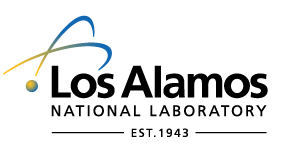
\includegraphics[trim=0.0in 0.0in 0.0in 0.0in,clip,height=0.18\textheight]{lanl-logo-footer.png} &
 \hspace{0.1em}
\includegraphics[height=0.18\textheight]{tamu_seal.png} &
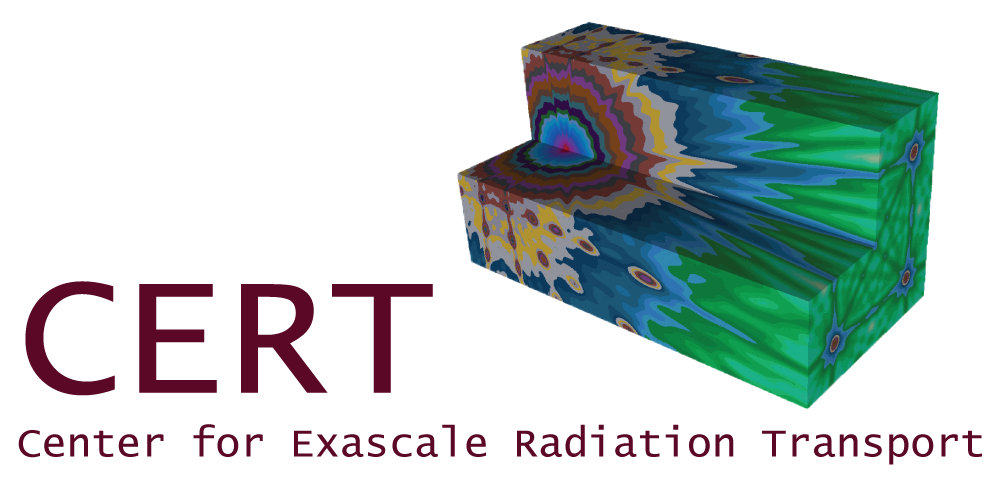
\includegraphics[height=0.18\textheight]{cert_logo_maroon.png}\end{tabular}}
%Michigan-themed
%\pgfdeclareimage[height=0.1in]{UMlogo}{michigan_engineering.png}
%\logo{\raisebox{-8pt}{\pgfuseimage{UMlogo}}}
%\titlegraphic{
\includegraphics[height=0.2\textheight]{michigan_block_m.png}}


%%%%%%%%%%%%%%%%%%%%%%%%%%%%%%%%%%%%%%%%%%%%%%%%%%%%%%%%%%%%%%%
% Optional packages, used to show off certain tricks

\newlength \figwidth
\setlength \figwidth {0.5\textwidth}


%%%%%%%%%%%%%%%%%%%%%%%%%%%%%%%%%%%%%%%%%%%%%%%%%%%%%%%%%%%%%%%

\usepackage[english]{babel}
\usetheme{boxes}

%Make it Aggie Maroon
\usecolortheme[RGB={80,0,0}]{structure}  
%Or Michigan Blue
%\usecolortheme[RGB={0,0,153}]{structure}  
%Or Michigan Maize
%\usecolortheme[RGB={255,204,0}]{structure}  


\setbeamertemplate{headline}{}
\setbeamertemplate{navigation symbols}{}%remove navigation symbols
\setbeamertemplate{footline}[frame number]



\setbeamersize{text margin left=1cm}
\setbeamersize{text margin right=0.75 cm}

\makeatletter
\let\old@rule\@rule
\def\@rule[#1]#2#3{\textcolor{rulecolor}{\old@rule[#1]{#2}{#3}}}
\makeatother

\definecolor{rulecolor}{RGB}{80,0,0}


  % This will typeset only the frames (or slides) that have the given label ("current" in this case).

\title[HOLO for TRT]{Residual Monte Carlo Transport in Time with Consistent Low-Order Acceleration for \\  1D Thermal Radiative Transfer}
    \author[S.R. Bolding]{{Simon Bolding and  Jim Morel}}
    \date{\vspace{-0.1in}{April 17 2017} }
\subject{}
%\institute{Los Alamos National Laboratory}

% \classificationlevel{SECRET/RD}
% \transmissible{}

%\reportnum{\textcolor{blue}{SAMPLE TEMPLATE ONLY \\ Contains NO Classified
%Information}}

% \dissableframenumber
\begin{document}
\setbeamercolor*{title}{use=structure,fg=white,bg=structure.fg}
\setbeamertemplate{title page}[default][colsep=-4bp,rounded=true,shadow=true]

\def\beginpage{\null\vfill\bgroup
\offinterlineskip\leftskip=\z@}
\def\endpage{\egroup\eject}

\begin{frame}
    \titlepage \vspace{-0.213in}
    \begin{center}
    \end{center}    
\end{frame}

\setlength{\tabcolsep}{6pt}

\setbeamercolor*{frametitle}{fg=Black!78}


%%%%%%%%%%%%%%%%%%%%%%%%%%%%%%%%%%%%%%%%%%%%%%%%%%%%%%%%%%%%%%%%%%%%%%%%%%%%%%%%%%%%%%%%%
\begin{frame}
\frametitle{We are interested in modeling thermal radiation transport \\ in the high energy
    density physics regime}
{\addtolength{\leftmargini}{-0.2in}
    \addtolength{\wideitemsep}{0.08in}
\begin{itemize}
    \item[] Modeling materials under extreme conditions \\ \colG{Temperatures $\mathcal{O}(10^6)$ K or more, e.g., supernovae}
    \item[] Photon radiation transports through a material \\ 
        \colG{Significant \colb{energy}  may be exchanged}
 \item[] This work increases time-integration accuracy \\ \colG{of the radiation variable in optically thin regions}
    \end{itemize}}
\end{frame}


%%%%%%%%%%%%%%%%%%%%%%%%%%%%%%%%%%%%%%%%%%%%%%%%%%%%%%%%%%%%%%%%%%%%%%%%%%%%%%%%%%%%%%%%%
{\addtolength{\leftmargini}{-0.2in}
\begin{frame}
\frametitle{Our method has been applied to a simplified model:\\ the 1D
    frequency-integrated radiative transfer equations}
\setlength{\unitlength}{\textwidth}
\vspace{0.152in}
\begin{itemize}
    \item[] Energy balance equations for radiation and material. \\
            \colG{Radiation intensity $I(x,\mu,t)$, material 
            temperature $T(x,t)$}\vspace{-0.34in}
    \item[] \begin{align*}\label{ho_cont}
\hspace{-0.134in}
    \frac{1}{c}\pderiv{I}{t} + \mu \pderiv{I}{x} + \sigma_t I(x,\mu,t)
    &= \frac{\sigma_s \phi(x)}{4\pi} +  \frac{1}{4\pi} \sigma_a a c T^4,
  \\
  C_v \pderiv{T(x,t)}{t} &=  \highlight{\sigma_a \phi(x,t)} - \highlight{\sigma_a a c T^4}\\
\end{align*}
            \vspace{-0.54043in}
        \item[] TRT equations are \colb{nonlinear} and may be tightly coupled \\  
            \colG{Absorption cross section ($\sigma_a$) can be a strong function of $T$}
        \item[] As $\sigma_a\rightarrow 0$, the equations become linear \\ and
                the radiation uncouples from the material
\end{itemize}
\end{frame}
}

\begin{frame}
    \frametitle{We will compare our time-integration accuracy \\ to the \textbf{Implicit Monte Carlo} (IMC) method}
{\addtolength{\leftmargini}{-0.3in}
   \begin{itemize}
        \item[] TRT equations are often solved with IMC \\
            \colG{which partially linearizes the system over a time step}
        \item[] Linearized \emph{radiation} equation is integrated \colb{continuously}
            \\ \colG{via MC sampling and tracking in time}
            \pause
        \item[] We have extended a \colb{high-order low-order (HOLO)} method:  \\ 
            \begin{itemize}
            \vspace{0.02in}
                 \item[] Previously shown to be statistically efficient \\ in optically thick problems
                 \item[] Use MC time-integration for radiation terms \\ \colG{instead of pure backward Euler in time}
           \end{itemize}
   \end{itemize}
   }
\end{frame}


\begin{frame}<*>
    \frametitle{\shorttitle}
        \vspace{0pt}
        \begin{minipage}[c][0.6\textheight]{0.2\textwidth}
            \hspace{-2em}
\includegraphics[width=\textwidth]{tamu_seal.png}\hspace{1em}
            \rule[-0.3\textheight]{1pt}{0.8\textheight}
        \end{minipage}
    \vspace{0pt}
        \begin{minipage}[c][0.6\textheight]{0.74\textwidth}
\tableofcontents[
hideothersubsections,
sectionstyle=show,
subsectionstyle=hide
]
         \end{minipage}
\end{frame}

\section{Overview of HOLO approach}
\subsection{}

%%%%%%%%%%%%%%%%%%%%%%%%%%%%%%%%%%%%%%%%%%%%%%%%%%%%%%%%%%%%%%%%%%%%%%%%%%%%%%%%%%%%%%%%%
\begin{frame}
    \frametitle{We produce a nonlinear low-order system with high-order
    angular and temporal correction from MC transport solves}
    \setlength{\unitlength}{1mm}
    \begin{picture}(120,80)(0,-84)
    \put(-5,-15){
    \begin{minipage}[t]{1.1\textwidth}
        \begin{itemize}
\setlength\wideitemsep{0.2in}
            \item[] The \textbf{LO system} is space-angle-time moment equations,\\
                    \colG{on a fixed finite-element (FE) spatial mesh}
                \vspace{0.06in}
                {\scriptsize
                \begin{itemize}
                    \item Reduced dimensionality and HO closures\\
                         \colG{allows for solution with Newton's method}
                     \vspace{-0.05in}
                 \item \textbf{Output:} linear-discontinuous  $\phi^{n+1}(x)$ and $T^{n+1}(x)$,\\ 
                         \colb{Construct LDFE emission source}
                \end{itemize}
}\vspace{0.2in}
            \item[] The \textbf{HO system} is a pure-absorber transport problem
                \vspace{0.05in}
                {\scriptsize
                \begin{itemize}
                    \item Solved with residual Monte Carlo (RMC) \\ \colG{for
                            \emph{efficient} reduction of statistical noise }
                     \vspace{-0.05in}
                    \item \textbf{Output:} \colb{consistency terms} to close LO equations \\
                \end{itemize}
}
        \end{itemize}
    \end{minipage}

}
\end{picture}
\end{frame}


%\begin{frame}
%\frametitle{Our {high-order low-order (HOLO) method} \\  improves on several drawbacks of standard IMC}
%    \begin{center}
%{\footnotesize
%\begin{tabular}{p{0.5\textwidth} p{0.5\textwidth}} 
%    \multicolumn{1}{l}{\textbf{\normalsize Standard  IMC}} & \multicolumn{1}{l}{\textbf{\normalsize
%    HOLO Method}} \\ \hline [2pt]
%    \parbox{0.4\textwidth}{Large \colr{statistical noise} possible} & 
%    \parbox{0.5\textwidth}{RMC is \colb{efficient} for TRT} \\ [\tabsep]
% \parbox{0.4\textwidth}{{\color{red}Effective scattering} can make \\ MC tracking very expensive}
% & \parbox{0.4\textwidth}{MC solution has \colb{no
% scattering}} \\[\tabsep] 
% \parbox{0.5\textwidth}{Linearization can cause \colr{non-physical}\\ results  (maximum principle
% violations)} & \parbox{0.5\textwidth}{Fully \colb{implicit} time-discretization
% and \\ LO solution \colb{resolves nonlinearities}} \\[\tabsep] 
% \parbox{0.5\textwidth}{\colG{Reconstruction of linear emission shape limits artificial energy propagation}} &
% \parbox{0.5\textwidth}{Linear-discontinuous FE for $T(x)$ \\ \colb{preserving equilibrium diffusion limit} }
%\end{tabular}
%}
%\end{center}
%\end{frame}

%%%%%%%%%%%%%%%%%%%%%%%%%%%%%%%%%%%%%%%%%%%%%%%%%%%%%%%%%%%%%%%%%%%%%%%%%%%%%%%%%%%%%%%%%


\section{Residual Monte Carlo High-Order Solver}
\subsection{}

%%%%%%%%%%%%%%%%%%%%%%%%%%%%%%%%%%%%%%%%%%%%%%%%%%%%%%%%%%%%%%%%%%%%%%%%%%%%%%%%%%%%%%%%%%
%{\addtolength\leftmargini{-0.165in}
%\begin{frame}
%    \frametitle{Exponentially Convergent Monte Carlo \\ can efficiently reduce noise globally}
%    \begin{itemize}
%            \addtolength{\wideitemsep}{0.14in}
%        \item[] Each MC batch tallies the \colb{error} in the solution 
%            \begin{itemize}
%                \item \colG{standard MC particle transport,\\ but a \colr{complex} source}
%                    \vspace{-0.21in}
%                \item \colG{RMC requires  a \colr{functional} representation of $I(x,\mu)$}
%    \end{itemize}
%
%        \item[] Can reduce solution error \colb{globally} $\propto e^{-\alpha N}$ \\
%            \colG{Adaptive $h$-refinement can help represent error}
%        \item[] $I^{n}(x,\mu)$ often provides an \colb{\textbf{excellent}} estimate of
%            $I^{n+1}(x,\mu)$\\  \colG{No MC sampling from thermal equilibrium regions}
%     \end{itemize}
% \end{frame}
% }



%%%%%%%%%%%%%%%%%%%%%%%%%%%%%%%%%%%%%%%%%%%%%%%%%%%%%%%%%%%%%%%%%%%%%%%%%%%%%%%%%%%%%%%%%
%{\addtolength\leftmargini{-0.165in}
%\begin{frame}
%    \frametitle{Residual Monte Carlo (RMC) \\ can efficiently reduce noise globally}
%    \begin{itemize}
%            \addtolength{\wideitemsep}{0.14in}
%        \item[] Each MC batch tallies the \textbf{error} in solution estimate
%            \begin{itemize}
%                \item A \colr{complex} residual source \\ \colG{with standard MC particle transport}
%                    \vspace{-0.21in}
%                \item {Residual requires  a \colr{functional} representation} \\ \colG{for all phase space variables being sampled}
%    \end{itemize}
%    \vspace{-0.1in}
%        \item[] We can not maintain exponential convergence \\
%       \colG{without adaptive $h$-refinement of trial space}    
%        \item[] We still gain efficiency from \colb{residual formulation} \\ with previous intensity as initial guess each time step
%     \end{itemize}
% \end{frame}
% }


%%%%%%%%%%%%%%%%%%%%%%%%%%%%%%%%%%%%%%%%%%%%%%%%%%%%%%%%%%%%%%%%%%%%%%%%%%%%%%%%%%%%%%%%%
\begin{frame}
    \frametitle{We apply the RMC algorithm to the HO transport eq., \\without discretization of the transport operator
    }
        \vspace{-0.05in}
        \begin{align*}
            \hspace{-0.2in}
            \left[\frac{1}{c}\pderiv{}{t} + \mu \pderiv{}{x} +
        \sigma_t\right]I(x,\mu,t)      &=  \frac{1}{4\pi}\left[\highlight{\sigma_a a c
    \left(T_{LO}^{n+1}\right)^4}\right]  \\[5pt]
            \B L \, I(x,\mu,t) &= q
     \end{align*}
     \pause
     \begin{block}{For each \textbf{batch} $m$:}
         \begin{itemize}
        \item Evaluate residual source: $r^{(m)} = q - \B L \tilde I^{n+1,(m)}$
        \item Estimate ${\epsilon}^{(m)} = \B L^{-1} {r}^{(m)}\;\;$ via \colb{MC simulation}    
 %       \item Update solution:\vspace{-0.08in} \begin{align*}\tilde I^{n+1,(m+1)} &= \tilde I^{n+1,(m)} + \tilde \epsilon^{(m)} \\ 
 %                                                 &= \colG{\tilde I^{n+1,(m)} + \B L^{-1} q - \B L^{-1} \B L \tilde
 %   I^{n+1,(m)}}\end{align*}
        \item Update solution: $\tilde I^{n+1,(m+1)} = \tilde I^{n+1,(m)} + \tilde \epsilon^{(m)}$
    \end{itemize}
\end{block}
\pause
     \begin{itemize}
        \item[] Initialize $\tilde I^((0))$  with previous intensity $\tilde I^{n-1/2}$\\ \colG{which is very efficient as optical thickness increases} 
        \end{itemize}
\end{frame}


%%%%%%%%%%%%%%%%%%%%%%%%%%%%%%%%%%%%%%%%%%%%%%%%%%%%%%%%%%%%%%%%%%%%%%%%%%%%%%%%%%%%%%%%%
 \begin{frame}
 \frametitle{RMC uses a \colb{projection} $\tilde I(x,\mu,t)$ onto a \\
 space-angle-time FE mesh to represent the solution}
    {\addtolength{\leftmargini}{-1.7cm}
     \begin{itemize}
         \item[] Linear-discontinuous (LD) FE projection in $x$ and $\mu$
         \item[] Tried three different $t$ spaces:  step-doubly discontinuous (SDD), \\ linear doubly-discontinuous (LDD), LD
            \end{itemize}
\begin{figure}[h]
    \centering
    \begin{subfigure}{0.42\textwidth}
    \centering
        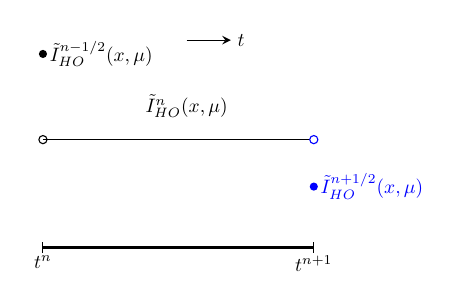
\begin{tikzpicture}[scale=0.702, every node/.style={transform shape}]
            \draw (1.0,4.0) node[fill,circle,inner sep=0pt,minimum
            size=4.2pt] {};
            \node[anchor=west] at (1.0,4.0) {${\tilde{I}_{HO}^{n-1/2}(x,\mu)}$};
            \draw [->] (3.6,4.25) -- (4.4,4.25) node[anchor=west] {$t$};
            \draw (1.0,0.4) -- (1.0,0.6) node[below, pos=0.4] {$t^{n}$};
            \draw (5.90,0.4) -- (5.90,0.6) node[below, pos=0.4] {$t^{n+1}$};
            \node at (3.6,3.06) {$\tilde{I}^n_{HO}(x,\mu)$};
            \draw [thick] (1.0,0.5) -- (5.9,0.5) node[anchor=north west] {};
            \filldraw[color=black, fill=white] (1,2.450) circle (2.1pt);
            \draw (1.0,2.45) -- (5.90,2.45);
            \filldraw[color=blue, fill=white] (5.9,2.450) circle (2.1pt);
            \draw (5.9,1.6) node[blue,fill,circle,inner sep=0pt,minimum size=4.2pt] {};
            \node[anchor=west] at (5.9,1.6) {\colb{${\tilde{I}_{HO}^{n+1/2}(x,\mu)}$}};
        \end{tikzpicture}
    \caption{\label{fig:sdd}SDD trial space}
    \end{subfigure}
    \hspace{0.4in}
    \begin{subfigure}{0.42\textwidth}
    \hspace{0.3in}
    \centering
    \vspace{0.1in}
        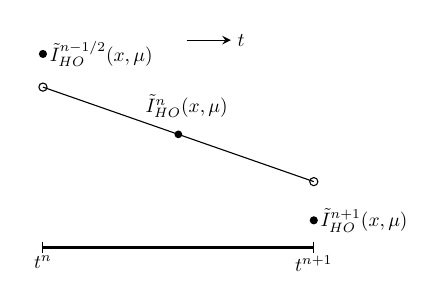
\begin{tikzpicture}[scale=0.702, every node/.style={transform shape}]
            \draw (1.0,4.0) node[fill,circle,inner sep=0pt,minimum
            size=4.2pt] {};
            \node[anchor=west] at (1.0,4.0) {${\tilde{I}_{HO}^{n-1/2}(x,\mu)}$};
            \draw (3.45,2.545) node[fill,circle,inner sep=0pt,minimum size=4.0pt] {};
            \draw [->] (3.6,4.25) -- (4.4,4.25) node[anchor=west] {$t$};
            \draw (1.0,0.4) -- (1.0,0.6) node[below, pos=0.4] {$t^{n}$};
            \draw (5.90,0.4) -- (5.90,0.6) node[below, pos=0.4] {$t^{n+1}$};
            \node at (3.6,3.06) {$\tilde{I}_{HO}^{n}(x,\mu)$};
            \filldraw[color=black, fill=white] (5.9,1.69) circle (2.1pt);
            \draw [thick] (1.0,0.5) -- (5.9,0.5) node[anchor=north west] {};
            \filldraw[color=black, fill=white] (1,3.40) circle (2.1pt);
            \draw (1.0,3.40) -- (5.90,1.69);
            \draw (5.9,0.99) node[black,fill,circle,inner sep=0pt,minimum size=4.2pt] {};
            \node[anchor=west] at (5.9,0.99) {${\tilde{I}_{HO}^{n+1}(x,\mu)}$};
        \end{tikzpicture}
        \caption{\label{fig:ld}LDD trial space}
    \end{subfigure}
\end{figure}
}
\end{frame}

%{\small
%    \begin{minipage}[c]{0.9\linewidth}
%        \vspace{33pt}
%             \begin{equation*}
%                 \tilde{I}_{ij}(x,\mu) = \  \tikzmark{moma}{\colb{I_{a}}}\ + \frac{2}{h_x}\;\tikzmark{momx}{\colb{I_{x}}}\  (x-x_i) +
%                 \frac{2}{h_\mu} \  \tikzmark{mommu}{\colb{I_{\mu}}}\  (\mu-\mu_i)
%             \end{equation*}
%        \begin{tikzpicture}[overlay, remember picture]
%    \node (descr) at (4,1.8) {local volumetric tallies};
%    \draw[,->,thick,Gray!60] (descr) to [in=90,out=-90] (moma);
%    \draw[,->,thick,Gray!60] (descr) to [in=90,out=-90] (momx);
%    \draw[,->,thick,Gray!60] (descr) to [in=90,out=-90] (mommu);
%        \end{tikzpicture}
%    \end{minipage}
%}
%    \end{itemize}
%\vspace{0.1in}
%   { \setlength\unitlength{1mm}
%    \begin{picture}(130mm,40mm)
%    \put(-4,40){
%    \begin{minipage}[t]{0.6\linewidth}
%        \vspace{0pt}
%        \centering
%        \scalebox{0.7}{
%        \begin{tikzpicture}
%            \hspace{-0.5in}
%            \draw (1,1) rectangle (4,4);
%            \node[draw,circle,inner sep=1.2 pt,fill] at (2.5,2.5) {};
%            \node[above] at (2.5,2.5) {$(x_i,\mu_j)$};
%            \node at (2.5,5.0) {Each $x$-$\mu$ cell};
%            \draw (1.0,0.4) -- (1.0,0.6) node[below, pos=0.4] {$x_{i-1/2}$};
%            \draw (4.0,0.4) -- (4.0,0.6) node[below, pos=0.4] {$x_{i+1/2}$};
%            \draw (0.4,1.0) -- (0.6,1.0) node[left, pos=0.4] {$\mu_{j-1/2}$};
%            \draw (0.4,4.0) -- (0.6,4.0) node[left, pos=0.4] {$\mu_{j+1/2}$};
%            \draw [thick,->] (0.5,0.5) -- (5,0.5) node[anchor=north west] {$x$};
%            \draw [thick,->] (0.5,0.5) -- (0.5,5) node[anchor=east] {$\mu$};
%        \end{tikzpicture}
%    }
%    \end{minipage}} 
%    \put(55,0){\centering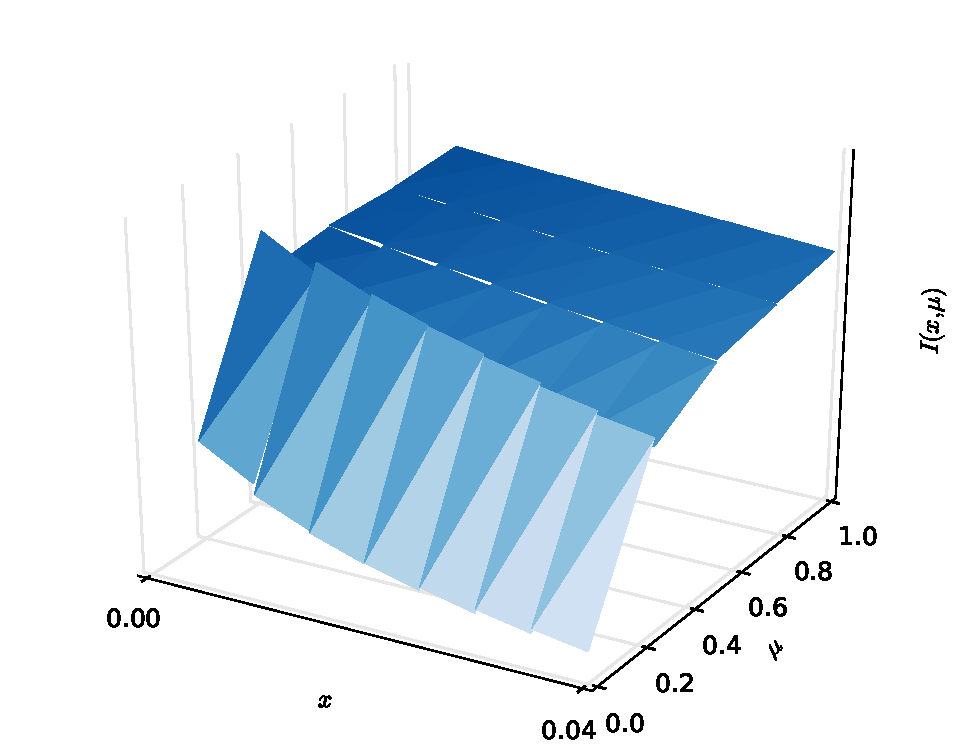
\includegraphics[trim=0.0in 0.0in 0.0in 0.5in,clip,width=0.55\textwidth]{zoom_angflux.pdf}
%        }
%    \end{picture}}
%\end{frame}




%%%%%%%%%%%%%%%%%%%%%%%%%%%%%%%%%%%%%%%%%%%%%%%%%%%%%%%%%%%%%%%%%%%%%%%%%%%%%%%%%%%%%%%%%
\begin{frame}
    \frametitle{We sample from a simplified FE residual source and\\ importance
    sampling estimates the residual magnitude}
    \addtolength{\wideitemsep}{0.05in}
    \begin{itemize}
        \item[] Cannot analytically evaluate L$_1$ norm of $x$-$\mu$-$t$ residual
            \\ \colG{because of 3D- and 2D-bi-linear functions }
        \item[] Sample from discontinuous, piece-wise constant approximation to PDF  $p^*(x,\mu,t)$:
           \begin{itemize}
            \item Values are quadrature approx. of L$_1$ norm \\ \colG{for each local volumetric- or $\delta$-function}
            \item Modified weights $w^*(x,\mu,t) = \frac{\ds r(x,\mu,t)}{\ds p^*(x,\mu,t)}$
            \end{itemize}
           \item[] Frequency of element samples $\propto$ $\|r\|_1$ over element,\\
               \colG{and this approach is extendable to higher dimensions}
        %\item[] Use cell-wise {systematic} sampling for $|r^{(m)}|$ source
    \end{itemize}
\end{frame}



\section{Derivation of the LO equations}
\subsection{}


%%%%%%%%%%%%%%%%%%%%%%%%%%%%%%%%%%%%%%%%%%%%%%%%%%%%%%%%%%%%%%%%%%%%%%%%%%%%%%%%%%%%%%%%%
\begin{frame}
    \frametitle{The LO equations are formed as \emph{consistently} as possible
        \\ with space-angle-time moments of TRT equations}
    \begin{itemize} \vspace{0.15in}
        \item[] Integration over time step $t \in [t^{n-1/2},t^{n+1/2}]$ \\ \colG{with implicit
            time discretization for temperature terms}
        \item[] Spatial moments are weighted with FE basis functions:   \end{itemize}
    \begin{columns}
        \begin{column}{0.5\textwidth}
    \begin{centering}
        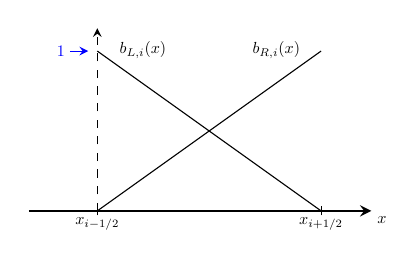
\begin{tikzpicture}[scale=0.58, every node/.style={transform shape}]
            \fill[fill=white] (11.0,0.5) rectangle (15.90,4.0);
            \node at (10.4,4.0) {$\colb{1}$ \hspace{0.8em} };
            \draw [Blue,->] (10.4,4.0) -- (10.8,4.0);
            \draw (11.0,0.4) -- (11.0,0.6) node[below, pos=0.4] {$x_{i-1/2}$};
            \draw (15.90,0.4) -- (15.90,0.6) node[below, pos=0.4] {$x_{i+1/2}$};
            \node at (14.92,4.02) {$b_{R,i}(x)$};
            \node at (12.0,4.02) {$b_{L,i}(x)$};
            \draw [thick,->] (9.5,0.5) -- (17.0,0.5) node[anchor=north west] {$x$};
            \draw [dashed,->] (11.0,0.5) -- (11.0,4.5);
            \draw (11.0,0.5) -- (15.90,4.0);
            \draw (15.90,0.5) -- (11.0,4.0);
        \end{tikzpicture}
    \end{centering}
        \end{column}
        \begin{column}{0.5\textwidth}
        \begin{equation*}
        \boxed{\displaystyle \mom{\cdot}_{L,i} = \frac{2}{h_i} \int_{x_\il}^{x_\ir}
        b_{L,i}(x)(\cdot) \d x \quad }  
        \end{equation*}
    \end{column}
\end{columns}
\begin{itemize}
        \vspace{0.2in}
    \item[] Half-range integrals reduce angular dimensionality
    \begin{equation*}
        \boxed{{\displaystyle \phi^+(x) =
        2\pi\int_0^1 I(x,\mu) \d \mu}}
    \end{equation*}
\end{itemize}
\end{frame}


%%%%%%%%%%%%%%%%%%%%%%%%%%%%%%%%%%%%%%%%%%%%%%%%%%%%%%%%%%%%%%%%%%%%%%%%%%%%%%%%%%%%%%%%%
\begin{frame}
    \frametitle{Apply moments to the TRT equations \\ and manipulate to form
        \colb{angular consistency
    terms}}
    {\addtolength{\leftmargini}{-1.2cm}
    \begin{itemize}
%        \item[] The streaming terms are algebraically manipulated \\ 
%            \colG{to form consistency terms (\colb{no approximation here})}
%            \vspace{0.3cm}
%            \pause
    \item[] Ultimately, we get six \textbf{exact} moment equations
             \\ \colG{for each spatial element $i$}
         \item[] For example, apply $\mom{\cdot}_{L,i}$ and $(\cdot)^+$ to streaming term \\ \colG{ and perform algebra to form angular averages}
    \end{itemize}$
    \fontsize{9.2}{13.0}\selectfont
    \begin{array}{lll}
        {\displaystyle\frac{h_i}{2} \left \langle \mu \pderiv{I}{x} \right \rangle_L^+ } & = &   
   \ds \frac{ 1}{ 2}\left[\mom{\mu I}_{L,i}^+ + \mom{\mu I}_{R,i}^+\right] - \left(\mu I \right)_{i-1/2}^+   \\
   & = & \ds \frac{1}{2} \left[\highlight{\frac{\ds\mom{\mu
        I}_{L,i}^+}{\ds\mom{I}_{L,i}^+}}\mom{I}_{L,i}^+  +
        \highlight{\frac{\ds\mom{\mu
    I}_{R,i}^+}{\ds\mom{I}_{R,i}^+}}\mom{I}_{R,i}^+\right]  - \highlight{\frac{\ds\left(\mu I
    \right)^+_{i-1/2} }{\ds I^+_{i-1/2}}}
        I^+_{i-1/2} 
            \end{array}$
    \begin{itemize}
            \vspace{0.2in}
            \item[] Now, approximate angular consistency terms \\ 
                with \colb{$\tilde I_{HO}(x,\mu,t)$} from previous HO solve
    \end{itemize}
}
\end{frame}


\begin{frame}
    \frametitle{The LO equations must be closed consistently \\ by eliminating $t^{n+1}$
unknowns with HO information}
    \begin{enumerate}
        \item Assume lumped-LDFE spatial closure \\\colG{ for $I^\pm(x)$, $T(x)$, \& $T^4(x)$}
    \item Eliminate space-angle moments of $I^{n+1/2}_{LO}$  in terms of
        \textbf{time-averaged} moments $\overline I_{LO}^n$, e.g.,
            \begin{equation*}
                \mom{I}_{L,i}^{n+1/2,+} = \highlight{\gamma^{HO,+}_{L,i}} {\mom{\overline{I}}}^{+,n}_{L,i} 
            \end{equation*}
        \item[] \colG{Coupled equations have same numerical complexity} \\ \colG{as a Backward Euler time-discretization}
        \pause
        \item After Newton solve for time-averaged moments, \\ use time closures to advance to the next time step
       \end{enumerate}
\end{frame}

\section{Summary of algorithm}


\begin{frame}
    \frametitle{For thin problems, which are nearly linear \\ one outer iteration is often sufficient}
    %\fontsize{9}{5.0}\selectfont
        \hspace{-0.1in}
        \resizebox{1.04\linewidth}{!}{
    \fontsize{10}{12.0}\selectfont
    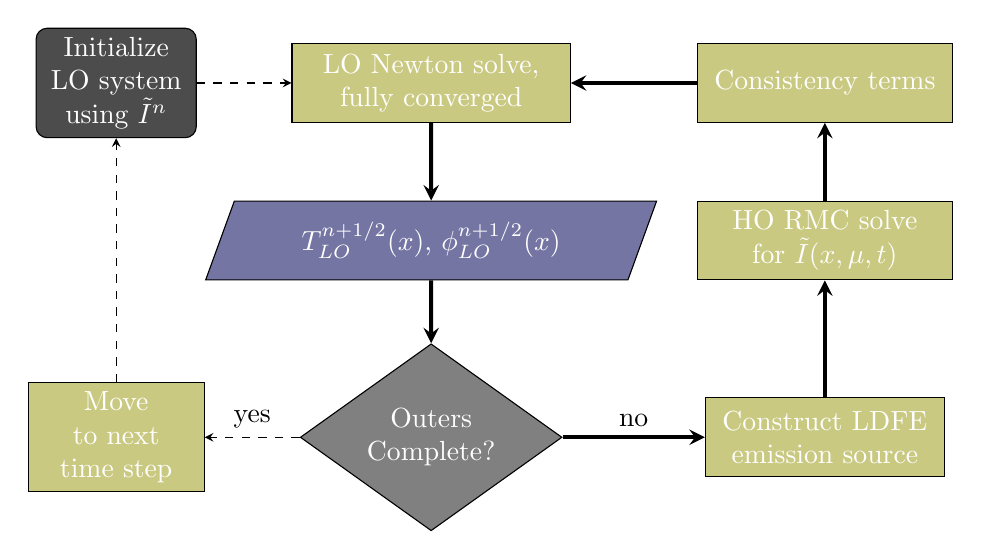
\begin{tikzpicture}[node distance=2cm]
        \node (start) [startstop] {Initialize LO system using $\tilde{I}^n$};
        \node (in1) [process, right of=start, xshift=2cm, text width=3.3cm]  {
        {LO Newton solve, fully converged}};
        \node (pro1) [io, below of=in1] {$T_{LO}^{n+1/2}(x)$, $\phi_{LO}^{n+1/2}(x)$};
        \node (dec1) [decision, below of=pro1, yshift=-0.5cm, text width=1.74cm] {Outers Complete?};
        \node (pro2a) [process, left of=dec1, xshift=-2.0cm] {Move to next time
        step};
        \node (srcs) [process, right of=dec1, xshift=3.0cm, text width=2.8cm] {
        {Construct LDFE emission source}};
        \node (pro2b) [process, text width=3.0cm, above of=srcs, yshift=0.5cm] {{HO RMC solve}
           for $\tilde I(x,\mu,t)$};
        \node (cons) [process, above of=pro2b, text width=3.0cm] {{Consistency
        terms}};
        \draw [arrow1] (start) -- (in1);
        \draw [arrow] (in1) -- (pro1);
        \draw [arrow] (pro1) -- (dec1);
        \draw [arrow] (srcs) -- (pro2b);
        \draw [arrow] (dec1.east) -- node[anchor=south] {no} (srcs);
        \draw [arrow1] (dec1.west) -- node[anchor=south] {yes} (pro2a);
        \draw [arrow1] (pro2a) -- (start);
        \draw [arrow] (pro2b) -- (cons);
        \draw [arrow] (cons) -- (in1);
    \end{tikzpicture}
}
\end{frame}

\section{Computational Results}
\subsection{}


\begin{frame}
    \frametitle{Implementation specifics for results are:}               
    {\addtolength\wideitemsep{11pt}
    \begin{itemize}
        \item {IMC results from Jayenne (LANL code)}
    \item One HO solve per time step, \\  with two LO solves
    \item Figure of Merit:  \boxed{\text{FOM}=\frac{\displaystyle 1}{\displaystyle
        \left(\frac{\ds\|\sigma(\phi_i)\|_2}{\ds\|\phi_i\|_2}\right)^2 N_{\text{total}}}}\\\vspace{0.05in} \colG{normalized so IMC FOM=1}
    \end{itemize}
    }
\end{frame}


\begin{frame}
    \frametitle{We will simulate several \textbf{Marshak Wave} problems \\ with different values for the absorption cross section}
    {\setlength\unitlength{1mm}
    \begin{picture}(150mm,80mm)(0,0)
    \put(0,20){
    \begin{minipage}[t]{\linewidth}
        \vspace{0pt}
        \begin{itemize}
            \item[] Figures depict radiation  \colb{temperature} $T_r = \sqrt[4]{\phi/ac}$ \\ or radiation \colb{energy-density} $E_r = \phi/c$
        \end{itemize}
    \end{minipage}} 
    \put(0,30){\centering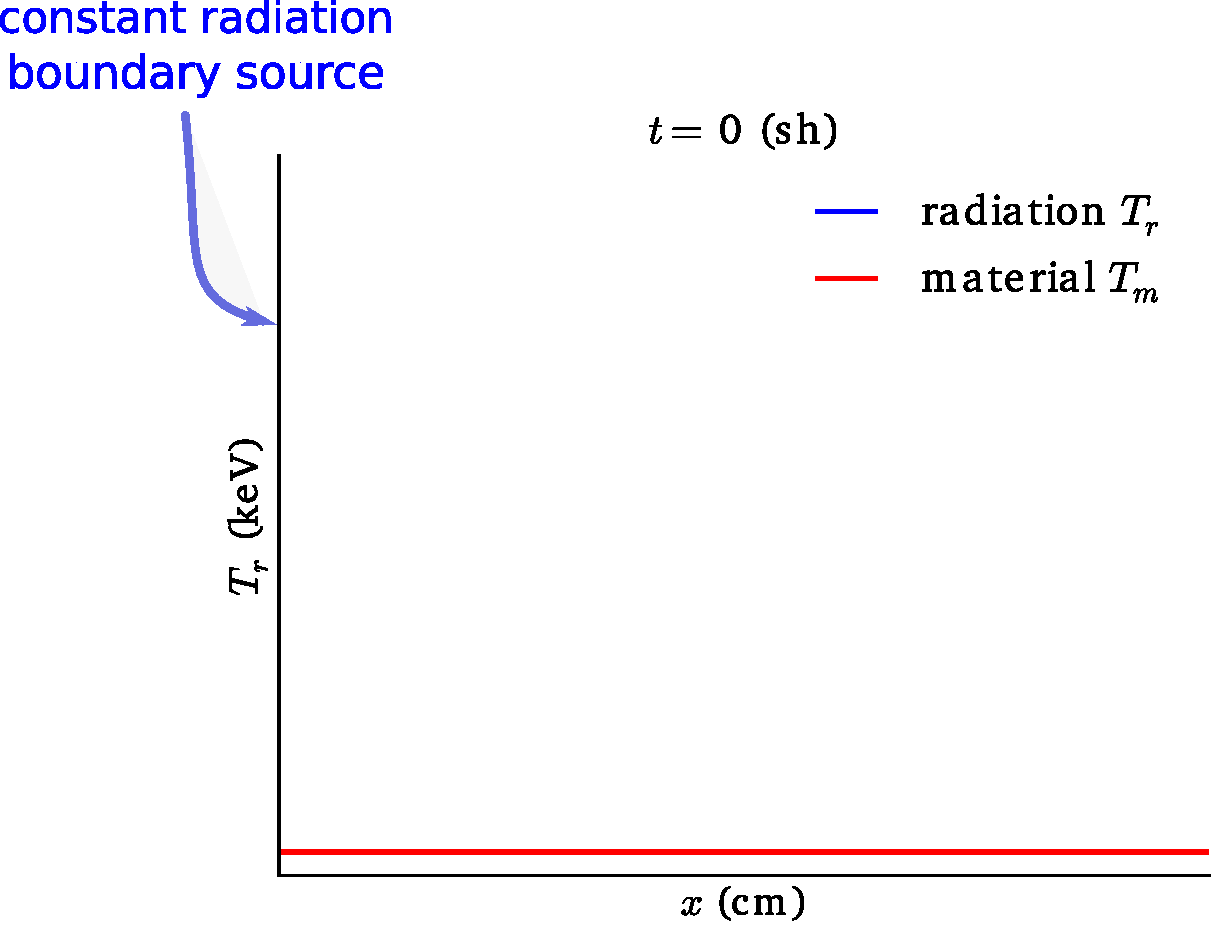
\includegraphics[trim=0.0in 0.0in 0.0in
    0.0in,clip,width=0.485\textwidth]{start_time_labeled.pdf}}
    \put(65,30){\centering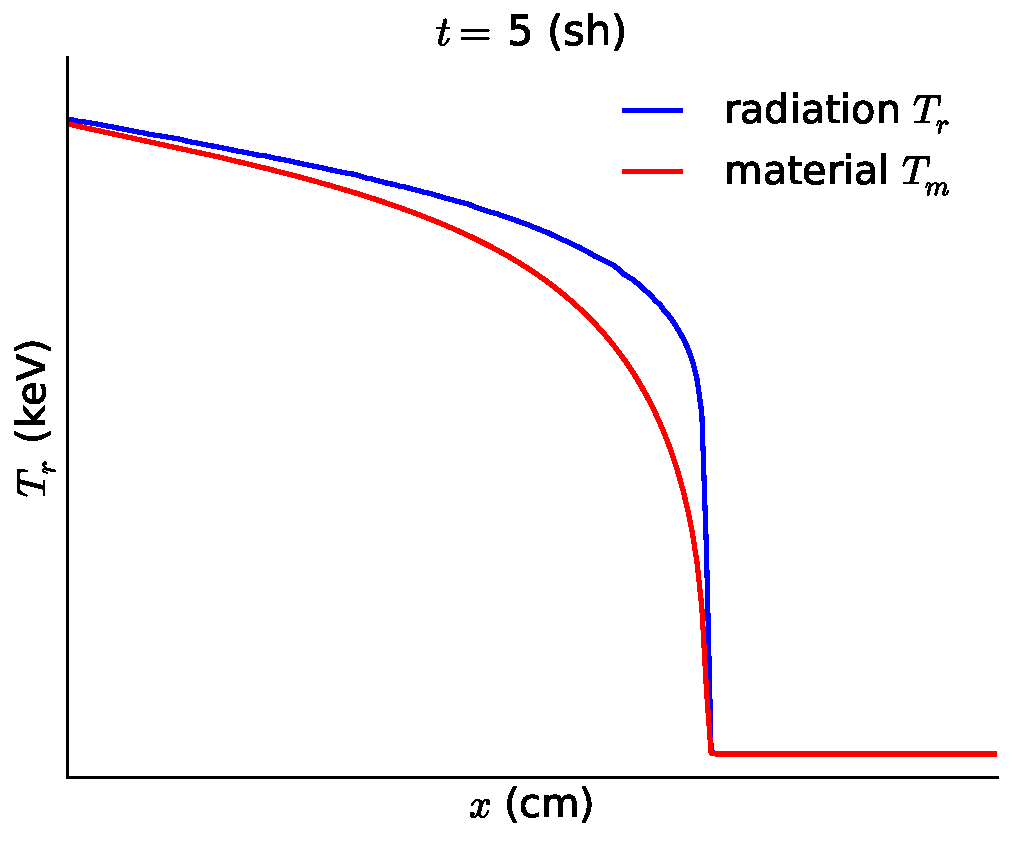
\includegraphics[trim=0.0in 0.0in 0.0in
    0.0in,clip,width=0.4\textwidth]{end_time.pdf}}
    \put(50,50){\tikz{\draw[->,line width=2mm,Gray!90] (0,0) -- (12mm,0);}}
\end{picture}}
\end{frame}

\begin{frame}
    \frametitle{HOLO can preserve accuracy of IMC \\ for near-void problem $\sigma_a=10^{-9}$ cm$^{-1}$}
    \begin{itemize}
    \vspace{0.1in}
        \item[] \textbf{Three} large time steps, $10^6$ histories per time step \\ \colG{Plots depict radiation energy densities $E_r=\phi(x)/c$}
        \item[] IMC is more efficient for this limiting case \\ \colG{because HOLO resamples intensity between time steps}
    \end{itemize}
        \begin{figure}
\centering
    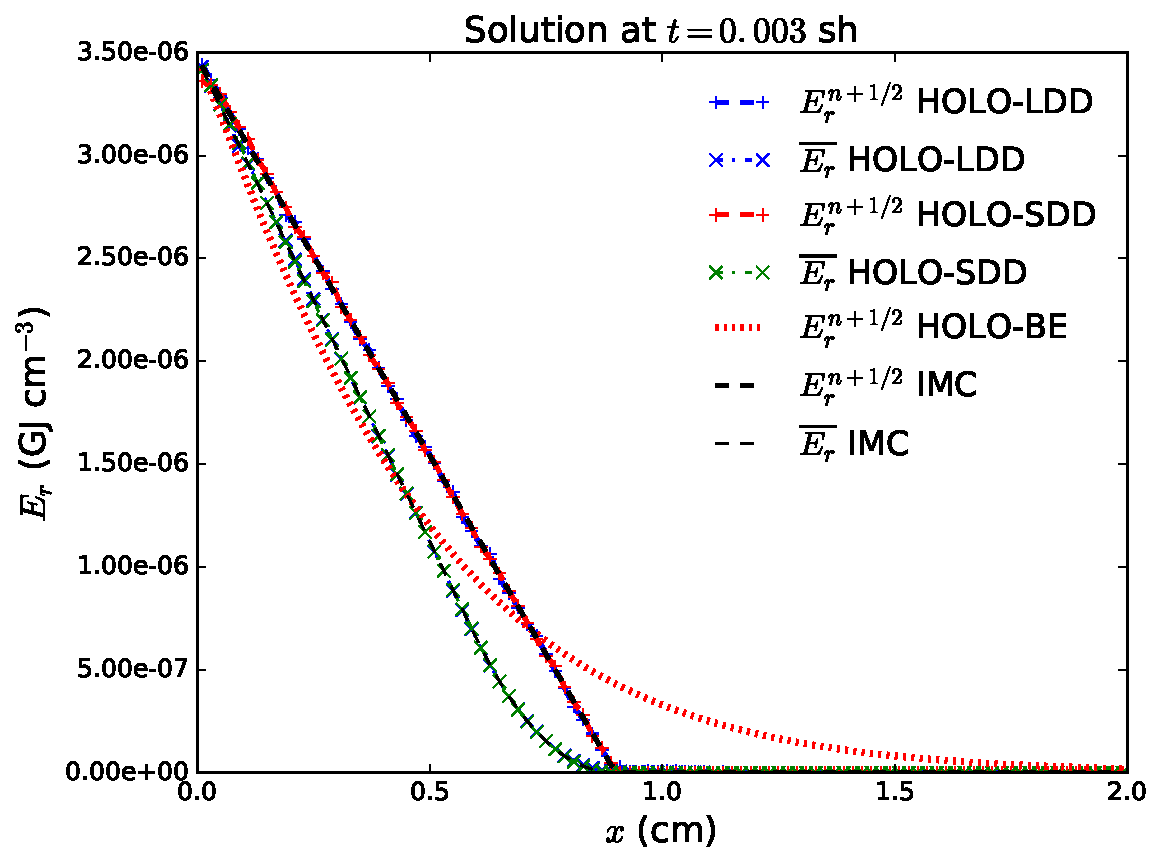
\includegraphics[width=0.6\textwidth]{void_imc_compare.pdf}
\end{figure}
\end{frame}

\begin{frame}
    \frametitle{The LDFE projection error between time steps \\ does not affect wave front location}
\begin{figure}[H]
  \centering
    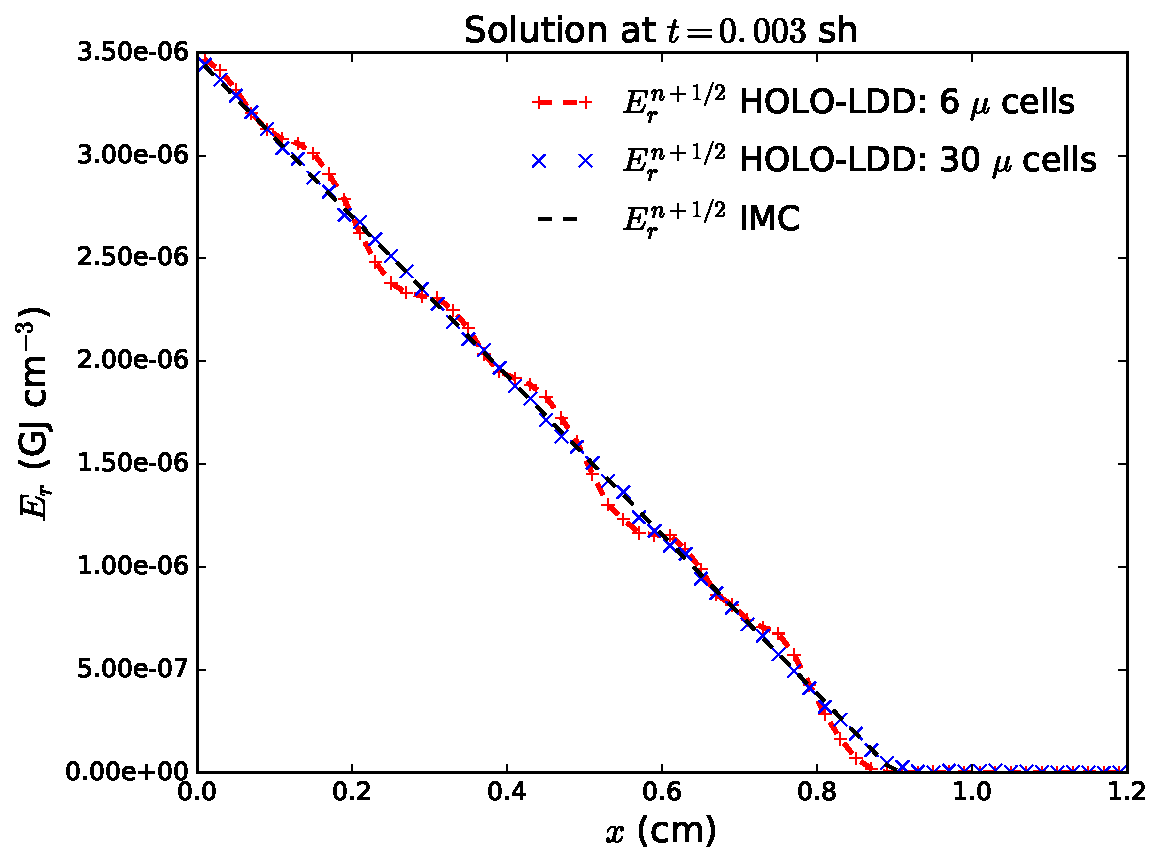
\includegraphics[width=0.75\textwidth]{void_ang_compare.pdf}
\end{figure}
\end{frame}


\begin{frame}
    \frametitle{The time closure preserves the accuracy \\ of MC time
    integration in LO solution} %Efficiency of time closure (HOLO-TC) \\ increases with optical thickness}
    \fontsize{10.0pt}{10.0pt}\selectfont
    \vspace{0.1in}
    \begin{itemize}
        \item Material has $\sigma_a = 0.2$ cm$^{-1}$, temperature mostly uncouples  \\
            \colG{Plots depict $T_{r}^{n+1}$ at $t=0.1$ sh}
        \item For HOLO w/ doubly-discontinuous spaces, smaller $\Delta t$ \\ decrease noise but increase projection error
        \item HOLO Backward Euler (HOLO-BE) is inaccurate
            \\ \colG{and HOLO-LD is unstable}
    \end{itemize}
\begin{figure}[H]
  \centering
    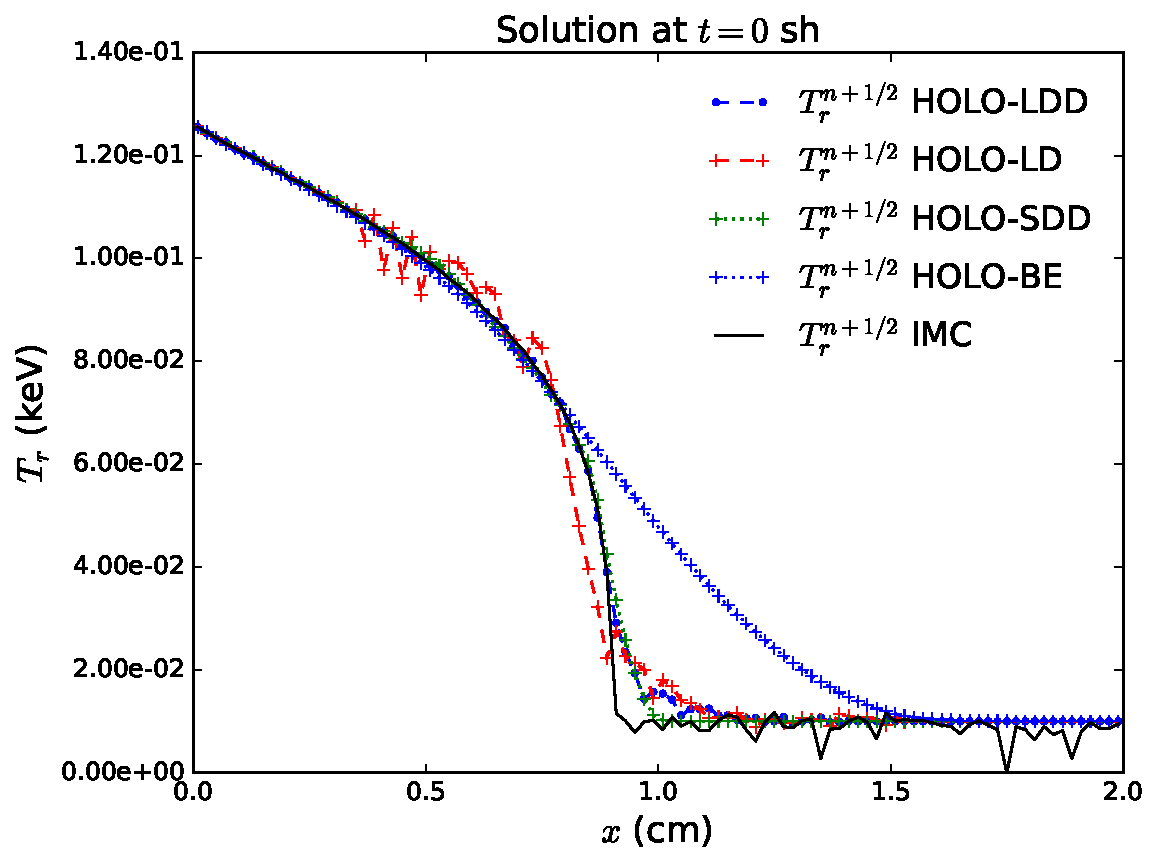
\includegraphics[width=0.590\textwidth]{thin_temp_compare.pdf}
\end{figure}
\end{frame}



\begin{frame}
    \frametitle{The HOLO method is more efficient than IMC \\ with a sufficiently fine space-angle mesh}
    \begin{itemize}
        \item Results for 200 $x$ cells, HOLO-TC has 60 $\mu$ cells \\ \colG{ $\Delta t =
            0.001$ sh}
        \item Error computed against IMC reference answer \\  with $4\times10^8$
            histories/step, 100 $x$ cells
    \end{itemize}
    \begin{table}
\begin{tabular}{|c|cc|cc|}\cline{2-5}
    \multicolumn{1}{c|}{}       & \multicolumn{2}{|c|}{$\mathbf{\|e_i\|_{2,rel}}$} &
    \multicolumn{2}{|c|}{\textbf{FOM}} \\ \hline
hists./step   & IMC     & HOLO-SDD (1) &    IMC   & HOLO-SDD(1)  \\ \hline
    30,000     & 2.93\%  & \colr{14.00\%}    & 1      &  \colr{unstable}      \\
    1,000,000   & 0.49\%  &\colb{ 0.18\% }   & 1.02   & \colb{ 81.7}      \\ \hline
\end{tabular}
\end{table}

\end{frame}

\begin{frame}
        \frametitle{The HO temporal closures are stable in a mix of thicknesses \\  with
    sufficient histories}
{\addtolength{\leftmargini}{-0.2in}
    \fontsize{9.0pt}{10.0pt}\selectfont
    \vspace{0.1in}
    \begin{itemize}
        \item Marshak wave problem, $\sigma \propto T^{-3}$, $10^6$ hists/step over 2 batches
    \end{itemize}
            \begin{figure}[H]
    \centering
    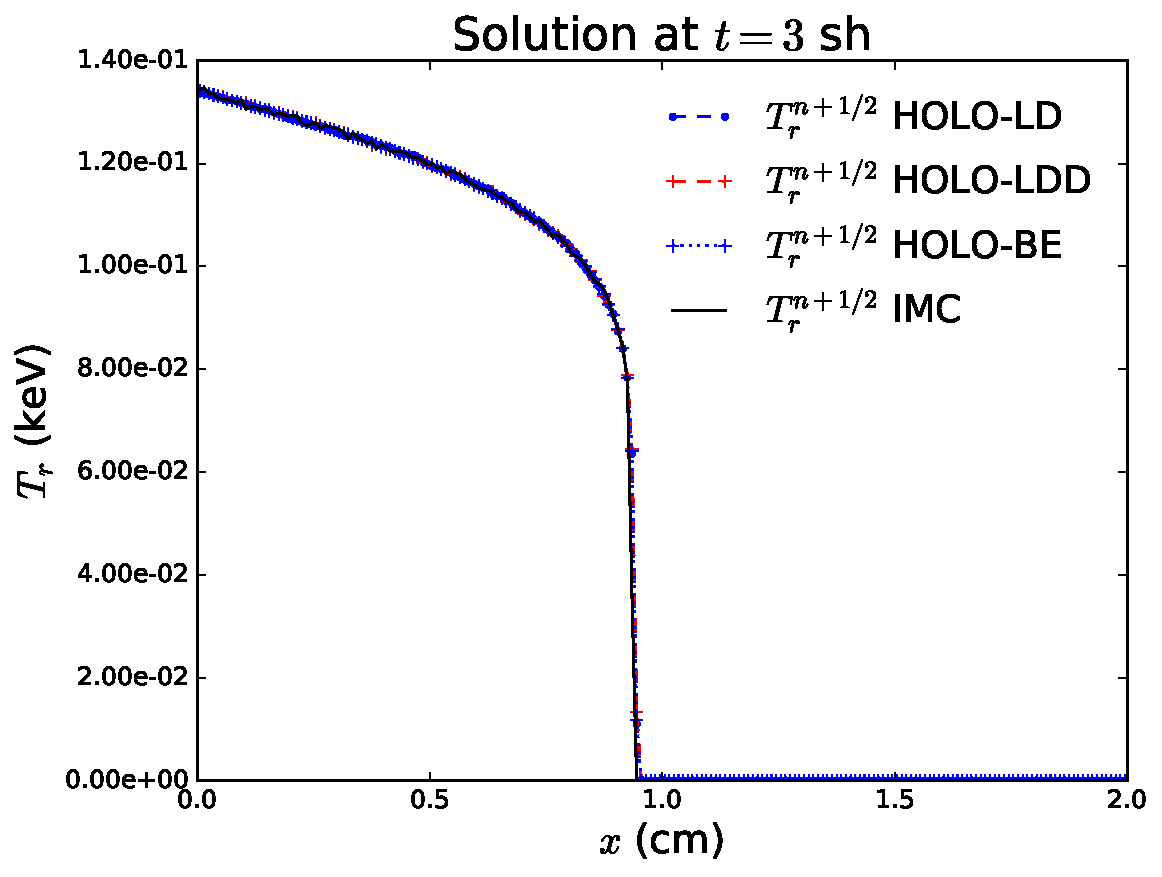
\includegraphics[width=0.56\textwidth]{marshak_time_cont_compare.pdf}
\end{figure}
\begin{itemize}
    \item Multiple batches are more efficent at estimating census
    \item HOLO-BE (FOM=1800) more efficient than HOLO-SDD (FOM=15) \\ but HOLO-LD (FOM=200) is comparable
    \end{itemize}
}
\end{frame}

\begin{frame}
    \frametitle{\shorttitle}
    \begin{itemize}
        \item[] RMC was extended to include the time variable\\
            \colG{and fits well in global HOLO context}
        \item[] HOLO method can be more efficient than IMC \\
            \colG{but would greatly benefit from $x$-$\mu$ adaptivity}
        \item[] The LO system is stable with sufficient statistics \\
            \colG{but the time-closure terms are not bounded}
        \item[] Next step is to extend to higher dimensions \\
            \colG{main hurdle to overcome is infrastructure}
    \end{itemize}
\end{frame}

\newcounter{finalframe}
\setcounter{finalframe}{\value{framenumber}}
\date{}

\begin{frame}
    \titlepage \vspace{-0.213in}
    \begin{center}
    \end{center}    
\end{frame}
\appendix
\title{Backup Slides}
\begin{frame}
    \vspace{-0.21in}
    \titlepage \vspace{-0.2113in}
\end{frame}

\title{Backup Slides}
\author{}
\date{}


\begin{frame}
\frametitle{Near-void problem plotted as radiation temperatures}
\begin{figure}
  \centering
    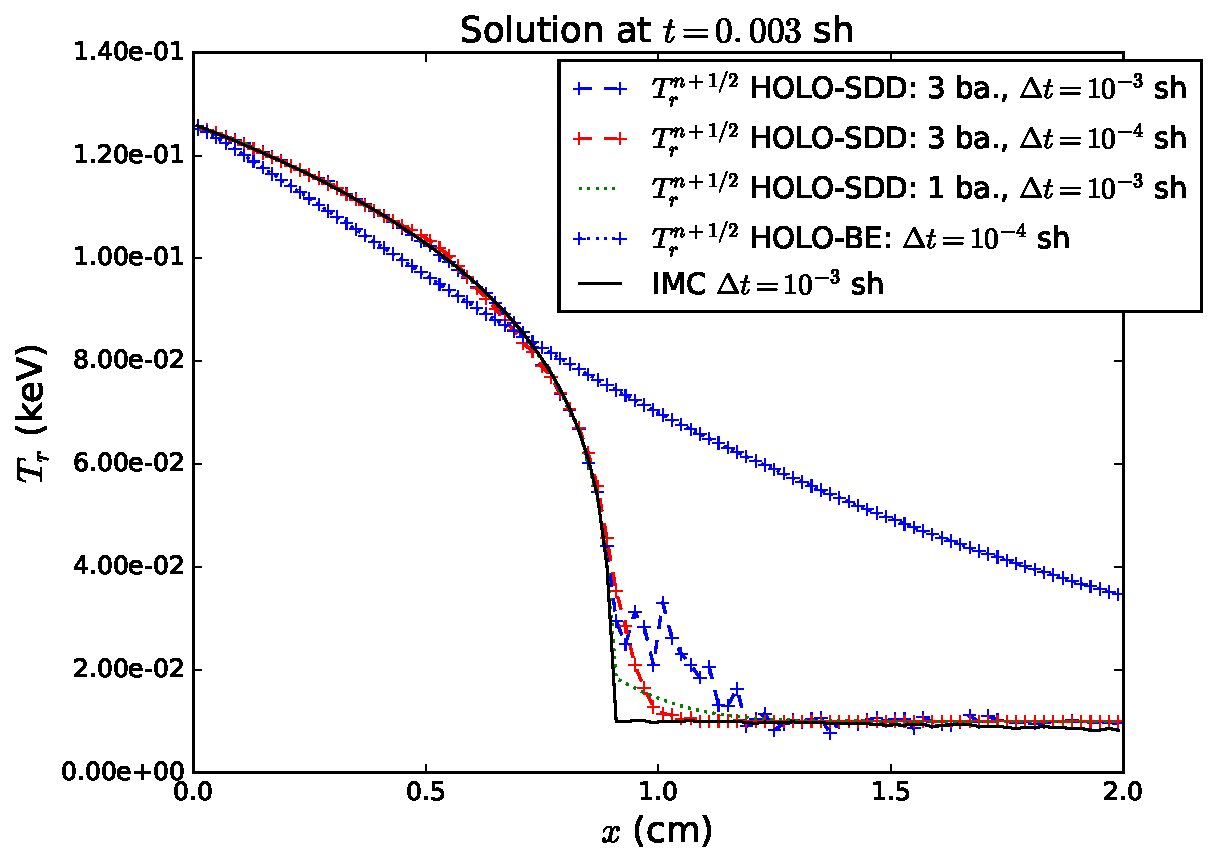
\includegraphics[width=0.5\textwidth]{void_temp_batch_compare.pdf}
\end{figure}
\end{frame}

\begin{frame}
    \frametitle{FOM and error norm definitions}
    Cell-averaged error norms
\begin{equation}
    \|e_i\|^{{(l)}}_{rel} = \left({\frac{\ds \sum\limits_{i=1}^{N^{(l)}_c}
    \left(\phi_i^{n+1,{(l)}} - \phi_i^{n+1,ref}
\right)^2}{\ds \sum\limits_{i=1}^{N^{(l)}_c}\left(\phi_i^{n+1,ref}\right)^2}}\right)^{1/2},
\end{equation}
FOM is based on the following variance
\begin{equation} 
    \sigma(\phi_i)^2 =  \frac{1}{N_{sim}-1} \sum_{l=1}^{N_{sim}} \left(\overline{\phi_{i}} -
    \phi_{i}^{(l)}\right)^2,
\end{equation}
\end{frame}

\begin{frame}
    \frametitle{RMC is more efficient than\\
 standard MC  as a HO solver }
{\addtolength\leftmargini{-0.345in}
    \centering
        \fontsize{10.0pt}{10.2pt}\selectfont
        \vspace{0.1in}
        \begin{itemize}
            \item Left half is optically thin ($\sigma\!=\!0.2$ cm$^{-1}$),
                right half is thick ($\sigma_a\!=\!2000$ cm$^{-1}$). \colG{8 $\mu$ cells,
                $\Delta t = 0.001$ sh}
            \item Results for HOLO with different HO solvers:\\
                \vspace{0.03in}\colb{ECMC} (FOM=10,000),  \colr{ standard MC}
                (FOM=0.46), and \colg{ S$_2$}
        \end{itemize}
    \begin{figure}
        \vspace{-0.1in} 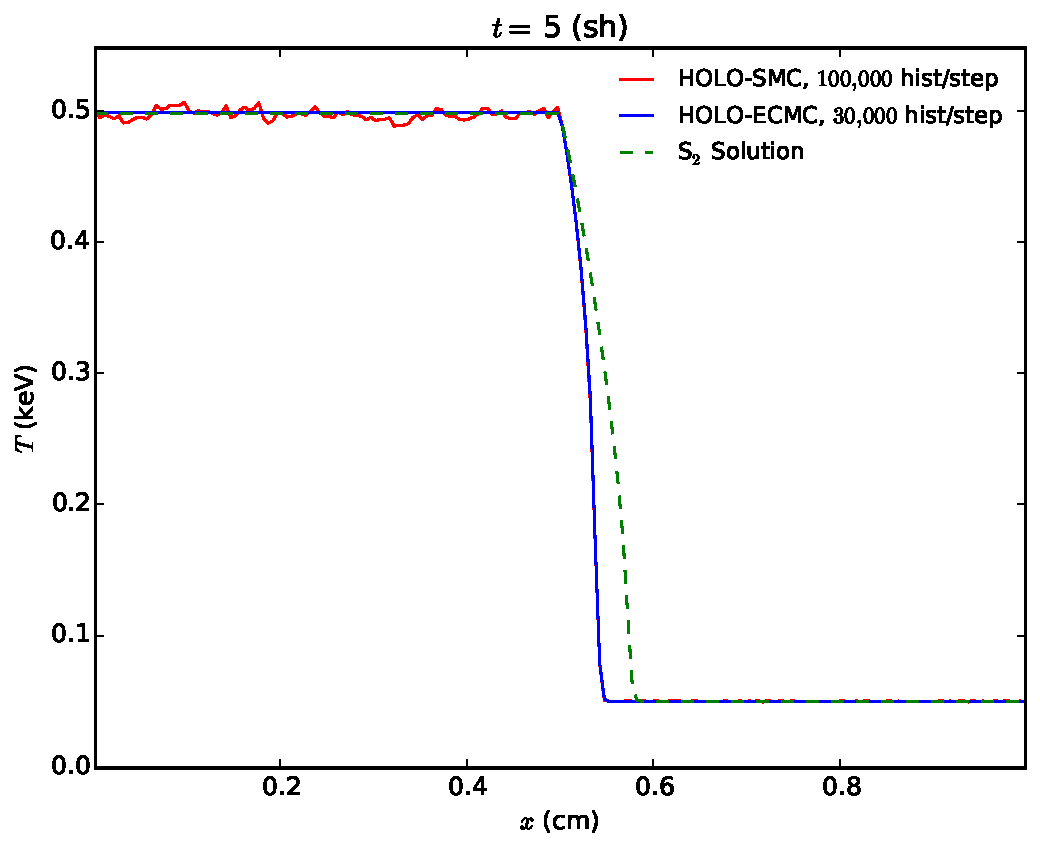
\includegraphics[width=0.6099\textwidth]{two_mat_ho_compare.pdf}
    \centering
    \end{figure}
}
\end{frame}

\begin{frame}
    \frametitle{Our HOLO method preserves 
                the maximum principle\\ with sufficient nonlinear convergence}
                {
                    \vspace{0.01in}
    \addtolength{\leftmargini}{-1.2cm}
                    \begin{itemize}
    \fontsize{9.62}{12.0}\selectfont
    \vspace{0.1in}
\item \textbf{Material temperatures} plotted; all simulations end at $t=0.1$ sh \\
    \colG{$\sigma_a \propto T^{-3}$, $c_v$ small, $\Delta t \in [10^{-4},10^{-2}]$ sh}  
                        \vspace{-0.1in}
            \item LO Newton iterations required damping 
        \end{itemize}
            }
    \vspace{0.0in}
                
    \hspace{0.62in}
    {\setlength\unitlength{1mm}
    \begin{picture}(130mm,80mm)(0,0)
    \put(21,74){\underline{{IMC $T_m$}} }
    \put(00,30){\centering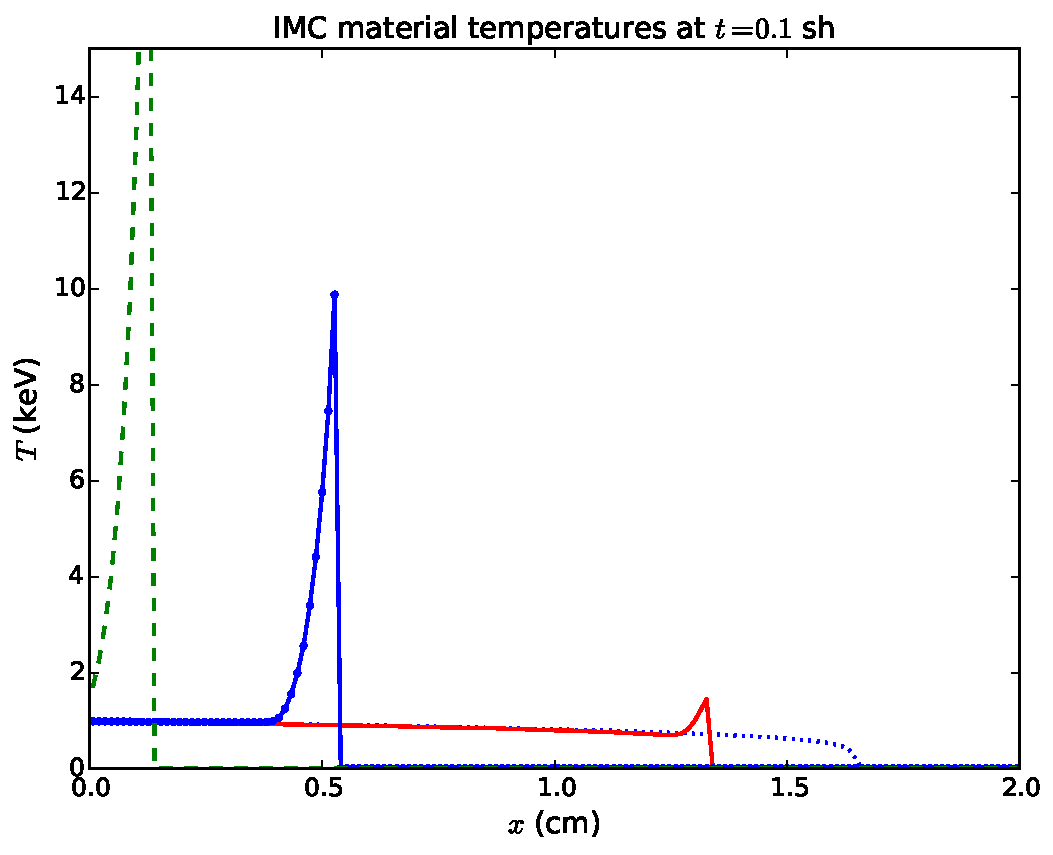
\includegraphics[trim=0.0in 0.0in 0.0in
    0.30in,clip,width=0.485\textwidth]{mpv_mats_imc_zoom.pdf}}
    \put(64.2,30){\centering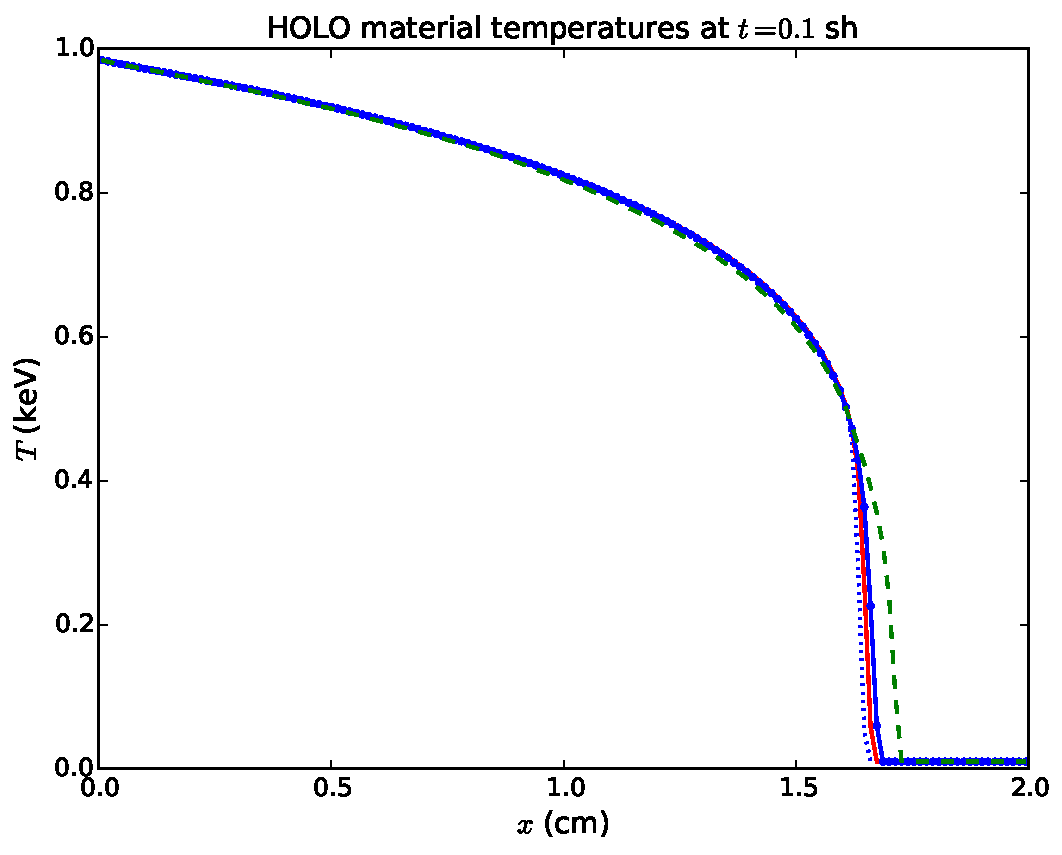
\includegraphics[trim=0.0in 0.0in 0.0in
    0.24in,clip,width=0.485\textwidth]{mpv_mats_holo_nolegend.pdf}}
    \put(85,74){\underline{{HOLO $T_m$}}}
    \put(30,40){\tikz{\draw[->,line width=0.3mm,black] (0,0) -- (-8mm,0);}}
    \put(28,42){\tiny $\Delta t$ increasing}
    \put(69,70.1){\tikz{\draw[fill=white,white] (0,0) rectangle (0.4\textwidth,2mm);}}
    \put(-7.8,36.0){\scriptsize {\color{Blue}$T_{r,\text{inc}}$}}
    \put(-0.7,36.5){\tikz{\draw[,->,line width=0.4mm,Blue] (20mm,0) -- (24mm,0);}}
    \put(56.5,69.3){\scriptsize {\color{Blue}$T_{r,\text{inc}}$}}
    \put(63.0,69.8){\tikz{\draw[,->,line width=0.4mm,Blue] (20mm,0) -- (23.5mm,0mm);}}
\end{picture}}
\end{frame}

\begin{frame}
    \frametitle{DSA allows for efficient iterative solution \\  of the low-order equations}
    \begin{itemize}
        \item[] Apply iterative solution methods to TRT two material problem
            with diffusivity of the thick region increased
    \end{itemize}
\begin{table}[p]
    \centering
    \begin{tabular}{c|c} \hline
        Method & Avg. Sweeps/Newton Iter. \\ \hline
        SI        & \colr{1037}      \\
        SI-DSA    & \colb{10.9}        \\
        GMRES     & 11.6        \\
        GMRES-DSA & \colb{6}      \\ \hline
    \end{tabular}
\end{table}
\begin{itemize}
    \item[]\colG{*25.1 \textbf{damped} Newton iterations per time step \\ Scattering iteration relative tolerance $10^{-10}$}
    \end{itemize}
\end{frame}

\begin{frame}
    \frametitle{The LDFE discretization of the LO equations \\ preserves the equilibrium diffusion limit}
                \vspace{0.05in}
        \begin{itemize}
            \item EDL Problem: \colG{Large, constant $\sigma_a$ and small $c_v$}
                \vspace{-0.1in}
            \item Apply HOLO algorithm, 12k histories per step
        \end{itemize}
\begin{figure}
    \centering
    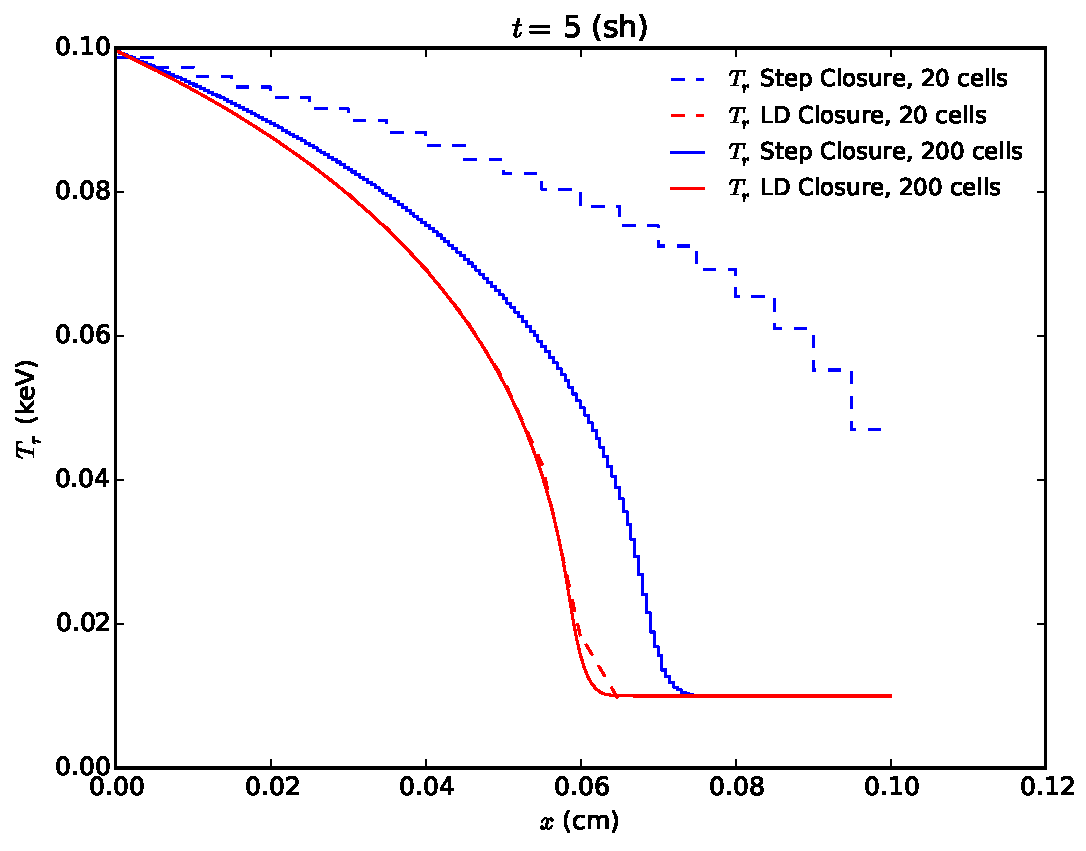
\includegraphics[width=0.6755799\textwidth]{diff_limit_compare.pdf}
\end{figure}
\end{frame}

\begin{frame}
    \frametitle{Implicit Monte Carlo (IMC) is the standard Monte Carlo transport method for TRT problems}
        \vspace{-0.2in}
\begin{itemize}
    \item[] The system is \emph{linearized} over a time step $t\in[t^n,t^{n+1}]$ \\ 
        \colG{Opacities are evaluated with $T(t^n)$}\vspace{0.21in}
\setlength\wideitemsep{0.2in}
    \begin{itemize}
        \item Produces a linear transport equation
               \\ \colG{with effective emission and scattering terms}
        \item MC particle histories are simulated 
            \\ \colG{tallying radiation energy deposition}
        \item Emission source is \textbf{not} fully time-implicit.\\
            \colG{Uses MC integration over $\Delta t$ for intensity}
    \end{itemize}
\end{itemize}
\end{frame}


\begin{frame}
    \frametitle{Time-integrated moment equation for $L$, $+$}
\begin{multline}\label{eq:t_moml_ex}
    \frac{\mom{\phi}_{L,i}^{+,n+1} - \mom{\phi}_{L,i}^{+,n}}{c \Delta t}
    -2\overline {\mu}_{i-1/2}^{\,+} \overline \phi_{i-1/2}^{\,+} + \overline{\cur {\mu}}_{L,i}^{+}
  \mom{\phibar}_{L,i}^{+}
  +  \overline{\cur\mu}_{R,i}^{+}
  \mom{\phibar}_{R,i}^{+}  \\ +   \sigma_{t,i}^{n+1} h_i 
  \mom{\overline\phi}_{L,i}^{n+1,+} -  \frac{\sigma_{s,i} h_i}{2} \left( \mom{\phibar}_{L,i}^{+} +
  \mom{\phibar}_{L,i}^{-}\right)  \\ = \frac{h_i}{2} \mom{\sigma_a^{n+1} a c T^{n+1,4}}_{L,i},
\end{multline}
\end{frame}



\begin{frame}
    \frametitle{Without sufficient histories, time closure can introduce instabilities}
\begin{figure}
    \centering
    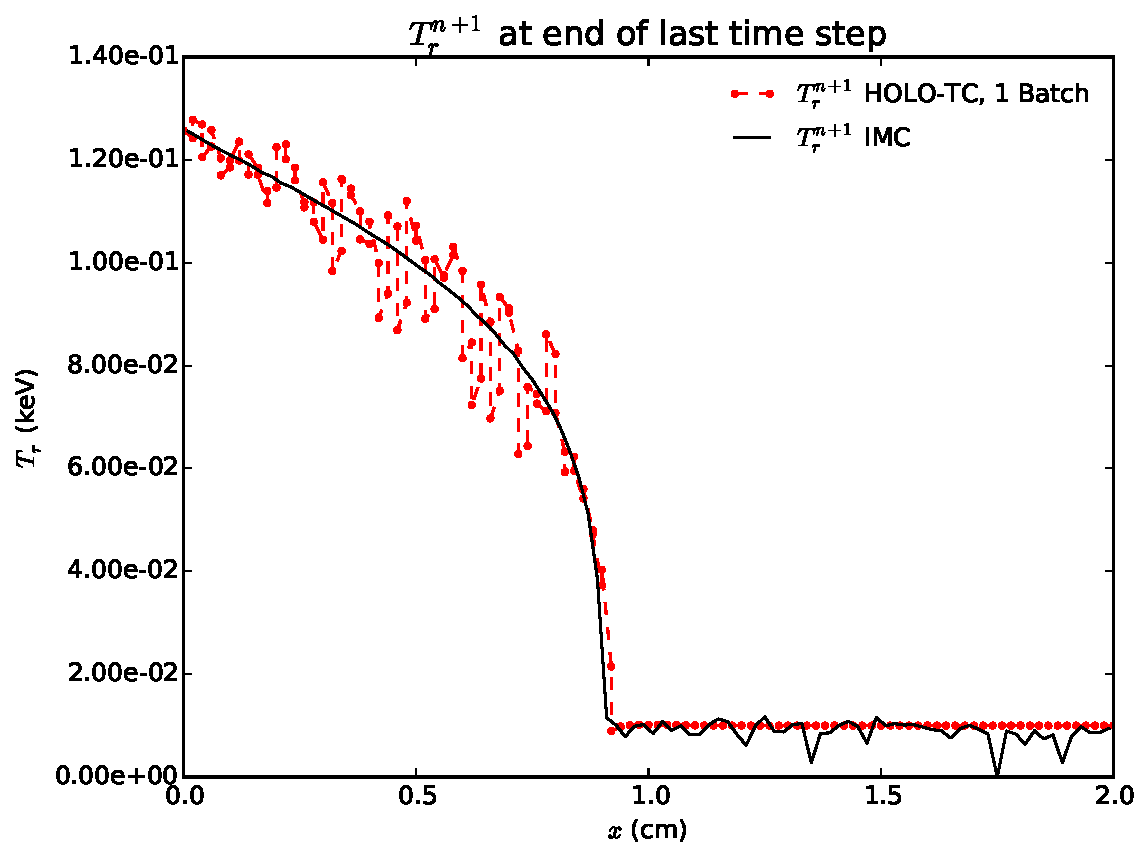
\includegraphics[width=0.75\textwidth]{thin_30k_fails.pdf}
\end{figure}
\end{frame}


%\begin{frame}
%    \frametitle{We will use a linear doubly-discontinuous (LDD) trial space  to allow for a HO
%        spatial closure}
%    \begin{columns}
%        \begin{column}[t]{0.2\textwidth}
%            \vspace{0pt}
%    \begin{center}
%        \begin{tikzpicture}[scale=0.62, every node/.style={transform shape}]
%            \draw (1.0,4.0) node[fill,circle,inner sep=0pt,minimum
%            size=4.2pt] {};
%            \draw [->] (1.6,4.25) -- (2.4,4.25) node[anchor=west] {$\mu$};
%            \draw (1.0,0.4) -- (1.0,0.6) node[below, pos=0.4] {$x_{i-1/2}$};
%            \draw (5.90,0.4) -- (5.90,0.6) node[below, pos=0.4] {$x_{i+1/2}$};
%            \node at (3.6,3.06) {$\phi_{LO}^+(x)$};
%            \draw [thick] (1.0,0.5) -- (5.9,0.5) node[anchor=north west] {};
%            \filldraw[color=black, fill=white] (1,3.1250) circle (2.1pt);
%            \draw (1.0,3.125) -- (5.90,2.120);
%            \filldraw[color=cyan, fill=white] (5.9,2.120) circle (2.1pt);
%            \draw (5.9,3.0) node[cyan,fill,circle,inner sep=0pt,minimum size=4.2pt] {};
%        \end{tikzpicture}
%    \end{center}
%    \end{column}
%    \begin{column}[t]{0.8\textwidth}
%    \vspace{0pt}
%    \begin{itemize}
%        \item $\tilde I_{HO}(x,\mu)$ will be linear in $\mu$ along face \\
%    \colG{Error estimated with MC face tallies}
%        \vspace{0.1in}
%        \item In LO equations use LDD for $\phi^{\pm}$\\
%             \colG{The linear interior preserves the EDL}
%        \vspace{0.1in}
%        \item Parameterize LO spatial closure to eliminate outflow:
%            \begin{equation*}
%                \phi^{+}_{i+1/2} = \frac{3+\highlight{\gamma_{i,HO}^+}}{2} \mom{\phi}_{R,i}^+ +
%                \frac{\highlight{\gamma^+_{i,HO}} - 3}{2}
%                \mom{\phi}_{L,i}^+
%            \end{equation*}
%    \end{itemize}
%    \end{column}      
%    \end{columns}
%\end{frame}

%%%%%%%%%%%%%%%%%%%%%%%%%%%%%%%%%%%%%%%%%%%%%%%%%%%%%%%%%%%%%%%%%%%%%%%%%%%%%%%%%%%%%%%%%




\setcounter{framenumber}{\value{finalframe}}
\end{document}
